\ac{GP}s are a Bayesian method for regression. We consider the regression input to be real-valued scalars $x_i$ and the regression output as the value of a function $f$ at $x_i$. The complete training data will be denoted by column vectors $\mathbf{x}$ and $\mathbf{f}$. Unseen test data is denoted with $\mathbf{\hat{x}}$ and $\mathbf{\hat{f}}$.
\ac{GP}s present a non-parametric way to express prior knowledge on the space of all possible functions $f$ modeling
a regression relationship.
Formally, a GP is an infinite-dimensional extension of the multivariate Gaussian distribution.
\begin{definition}
A Gaussian process (GP) is a collection of random variables, any
finite number of which have a joint Gaussian distribution~\citep[][chapter 2]{rasmussen2006gaussian}.
\end{definition}
The collection of random variables $\br{f(x)}$ (indexed by $x$) represents the
values of the function $f$ at each location $x$.
The \ac{GP} determines a Gaussian distribution over possible functions 
which is determined by a \ac{GP} mean function $m(x)$ and a covariance function or kernel $k(x,x^\prime)$.
We are going to derive expressions for the conditional mean and covariance of a
GP.  To simplify the calculations, we will assume prior mean zero; once the
derivation is done, this assumption can easily be relaxed via translation.

We write $\mathbf{K}(\xbf,\xbf^\prime)$ for the prior covariance matrix determined by $\xbf$ and $\xbf^\prime$, that
is, the covaricance between the random vectors $\{f(x\}_{x \in \xbf}$ and $\{f(x')\}_{x' \in
\xbf'}$.
 


The joint prior distribution of training and test output is defined as 
\begin{equation}
\begin{bmatrix}
\mathbf{f} \\ 
\mathbf{\hat{f}}
\end{bmatrix}
\sim \mathcal{N}\bigg(
0,
\begin{bmatrix}
K(\mathbf{x},\mathbf{x})& K(\mathbf{x},\mathbf{\hat{x}})\\ 
K(\mathbf{\hat{x}},\mathbf{x})& K(\mathbf{\hat{x}},\mathbf{\hat{x}})
\end{bmatrix}
\bigg).
\end{equation}
Since the joint distribution is Gaussian, the conditional is Gaussian, too
\begin{equation}
\label{eq:simple_posterior}
P(\hat{\mathbf{f}} \mid \mathbf{f})  = \frac{P(\hat{\mathbf{f}}, \mathbf{f}) }{P(\mathbf{f})}.
\end{equation}
This predictive posterior can be written as:

\begin{equation}
\label{eq:mackay_posterior}
P(\hat{\mathbf{f}} \mid \mathbf{f}) 
\propto \exp\bigg\{
\begin{bmatrix}
\mathbf{f} \; 
\mathbf{\hat{f}}
\end{bmatrix}
\begin{bmatrix}
K(\mathbf{x},\mathbf{x})& K(\mathbf{x},\mathbf{\hat{x}})\\ 
K(\mathbf{\hat{x}},\mathbf{x})& K(\mathbf{\hat{x}},\mathbf{\hat{x}})
\end{bmatrix}^{-1}
\begin{bmatrix}
\mathbf{f} \\ 
\mathbf{\hat{f}}
\end{bmatrix}
\bigg\}
\end{equation}
Instead of computing the inverse as above, we resort to write 

\begin{equation}
\begin{bmatrix}
K(\mathbf{x},\mathbf{x})& K(\mathbf{x},\mathbf{\hat{x}})\\ 
K(\mathbf{\hat{x}},\mathbf{x})& K(\mathbf{\hat{x}},\mathbf{\hat{x}})
\end{bmatrix}^{-1}
=
\begin{bmatrix}
\mathbf{M}& \mathbf{m}\\ 
\mathbf{m}^\top & \mathbf{\hat{K}}^{-1} 
\end{bmatrix}
\end{equation}
where we use using partionened inverse equations (\citealp*{barnett1979matrix} following \citealp*{mackay1998introduction}) with:
\begin{align}
\mathbf{\hat{K}} =& K(\mathbf{\hat{x}},\mathbf{\hat{x}}) -K(\mathbf{\hat{x}},\mathbf{x}) K(\mathbf{x},\mathbf{x})^{-1}K(\mathbf{x},\mathbf{\hat{x}}),\\
\mathbf{m} =& -\mathbf{\hat{K}}^{-1} \mathbf{K}(\mathbf{x},\mathbf{x}^{-1}) K(\mathbf{x},\mathbf{\hat{x}}),\text{ and}\\
\mathbf{M} =&  \mathbf{K}(\mathbf{x},\mathbf{x}^{-1}) + \frac{1}{\mathbf{\hat{K}}}\mathbf{m}\mathbf{m}^\top.
\end{align}
by substituting in \ref{eq:mackay_posterior}, we can write:
\begin{equation}
P(\hat{\mathbf{f}} \mid \mathbf{f}) 
\propto \frac{1}{Z} 
\exp\bigg\{
\frac{(\mathbf{\hat{f}} - (K(\mathbf{\hat{x}},\mathbf{x}) K(\mathbf{x},\mathbf{x})^{-1}\mathbf{f}))^2}{2(K(\mathbf{\hat{x}},\mathbf{\hat{x}}) -K(\mathbf{\hat{x}},\mathbf{x}) K(\mathbf{x},\mathbf{x})^{-1}K(\mathbf{x},\mathbf{\hat{x}}))}
\bigg\}.
\end{equation} 
In this expression, we simplify 
\begin{equation}
\bm{\hat{\mu}} = K(\mathbf{\hat{x}},\mathbf{x}) K(\mathbf{x},\mathbf{x})^{-1}\mathbf{f}
\end{equation}
so that for sampling from the predictive posterior, we can write:
\begin{equation}
\mathbf{\hat{f}} \mid \mathbf{\hat{x}},\mathbf{x},\mathbf{f} 
\sim \mathcal{N}(\bm{\hat{\mu}},\mathbf{\hat{K}}).
\end{equation}

Often one assumes the observed regression output is noisily measured, that is, one only sees the values of $\ybf_\noisy = \mathbf{f}+ \wbf$ where $\wbf$ is Gaussian white noise with variance $\sigma_\noise^2$. This noise term can be absorbed into the covariance matrix $\mathbf{K}(\mathbf{x},\mathbf{x})$ which in the following, we will write as $\mathbf{K}$ for readability. The log-likelihood of a \ac{GP} can then be written as:
\begin{equation}
\label{eq:gplogdens}
\log P(\mathbf{f} \mid \xbf) =
-\frac12 \ybf^\top 
\mathbf{K}^{-1} \ybf
- \frac12\log \abs{\mathbf{K}}
- \frac{n}{2}\log 2\pi
\end{equation}
where $n$ is the number of data points.
Both log-likelihood and predictive posterior can be computed efficiently using a \ac{SP} in Venture~\citep{mansinghka2014venture}
with an algorithm that resorts to Cholesky factorization\citep[chap. 2]{rasmussen2006gaussian}. 
We write the Cholesky factorization as 
$\mathbf{L} \coloneqq \text{chol}(\mathbf{K})$ when
:
\begin{equation}
\mathbf{K} = LL^\top
\end{equation}
where L is a lower triangular matrix. This allows us to compute the inverse of a covariance matrix as
\begin{equation}
\mathbf{K}^{-1} = (\mathbf{L}^{-1})^\top (\mathbf{L}^{-1})
\end{equation}
and its determinant as 
\begin{equation}
det(\mathbf{K}) = det(\mathbf{L})^2
\end{equation}
We compute (\ref{eq:gplogdens}) as
\begin{equation}
\log(P(\mathbf{f}\mid \mathbf{x})\coloneqq - \frac{1}{2} \mathbf{f}^\top \bm{\alpha} - \sum_i \log \mathbf{L}_{ii} - \frac{n}{2} \log 2 \pi
\end{equation}
where 
\begin{equation}
\label{eq:chol_L}
\mathbf{L} \coloneqq \text{chol}(\mathbf{K})
\end{equation}
and 
\begin{equation}
\label{eq:alpha}
\bm{\alpha} \coloneqq  \mathbf{L}^\top \backslash(\mathbf{L} \backslash \mathbf{f}). 
\end{equation}
This results in a computational complexity of $\mathcal{O}(n^3)$ in the number of data points for
sampling with a complexity of $n^3/6$ for (\ref{eq:chol_L}) an $n^2/2$ for (\ref{eq:alpha}). 

\begin{figure}
 \centering

     \begin{subfigure}[b]{0.45\textwidth}
        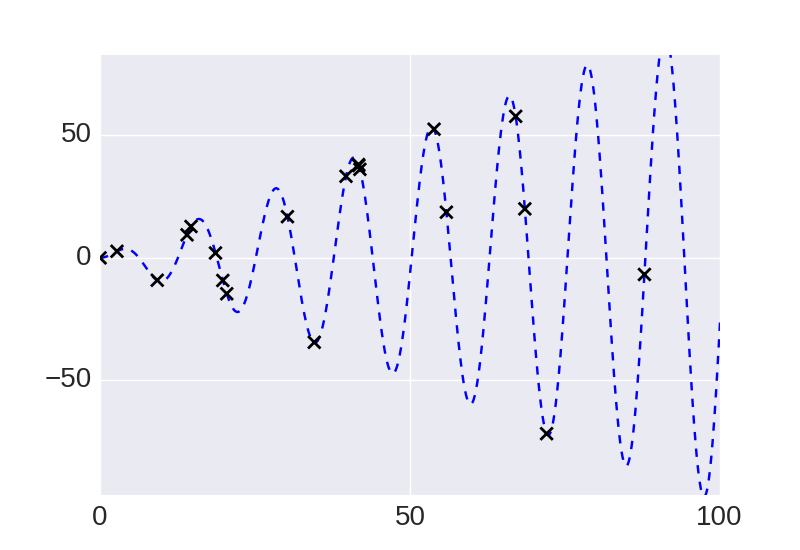
\includegraphics[width=\textwidth]{figs/composition/composition_demo_raw_data.png}
        \caption{Raw Data}
    \end{subfigure}
    ~ %add desired spacing between images, e. g. ~, \quad, \qquad, \hfill etc. 
      %(or a blank line to force the subfigure onto a new line)
    \begin{subfigure}[b]{0.45\textwidth}
\small
     \begin{align*}
    \text{LIN} &=   \sigma_1^2(x x^\prime)\\
    \text{PER} &=  \sigma_2^2 \exp \bigg( \frac{2 \sin^2 ( \pi (x - x^\prime)/p}{\ell^2} \bigg)\\ 
    \text{LIN} \times \text{PER} &=  \sigma_1^2(x x^\prime)\, \sigma_2^2 \exp \bigg( \frac{2 \sin^2 ( \pi (x - x^\prime)/p}{\ell^2} \bigg) 
    \end{align*}\vspace{5mm} 
        \caption{Kernels}
    \end{subfigure}\vspace{4mm} 


Parameterized Kernels:\vspace{3mm} 

     \begin{subfigure}[b]{0.3\textwidth}
      \centering \footnotesize
       $20.1^2(x x^\prime) $ \vspace{2mm}
	\caption{LIN}
    \end{subfigure}
    ~ %add desired spacing between images, e. g. ~, \quad, \qquad, \hfill etc. 
      %(or a blank line to force the subfigure onto a new line)
    \begin{subfigure}[b]{0.3\textwidth}
      \centering \footnotesize
      $19.1^2 \exp \bigg( \frac{2 \sin^2 ( \pi (x - x^\prime)/37.7}{6.3^2} \bigg)$ 
	\caption{PER}
    \end{subfigure}
    ~ %add desired spacing between images, e. g. ~, \quad, \qquad, \hfill etc. 
    %(or a blank line to force the subfigure onto a new line)
    \begin{subfigure}[b]{0.3\textwidth}
    \centering \footnotesize
      $383.9^2 (x x^\prime) \exp \bigg( \frac{2 \sin^2 ( \pi (x - x^\prime)/37.7}{6.3^2} \bigg)$ 
        \caption{LIN $\times$ PER}
    \end{subfigure} \vspace{4mm} 

Prior:

     \begin{subfigure}[b]{0.3\textwidth}
        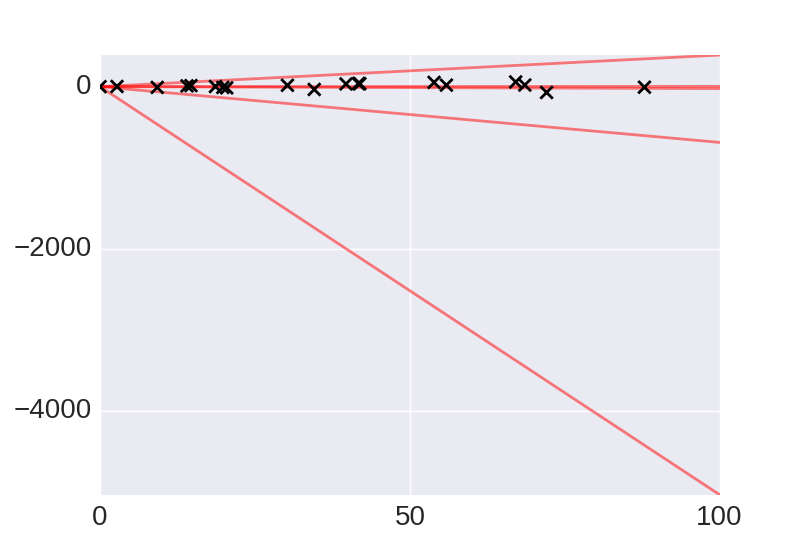
\includegraphics[width=\textwidth]{figs/composition/composition_demo_LIN_prior.png}
        \caption{LIN}
    \end{subfigure}
    ~ %add desired spacing between images, e. g. ~, \quad, \qquad, \hfill etc. 
      %(or a blank line to force the subfigure onto a new line)
    \begin{subfigure}[b]{0.3\textwidth}
        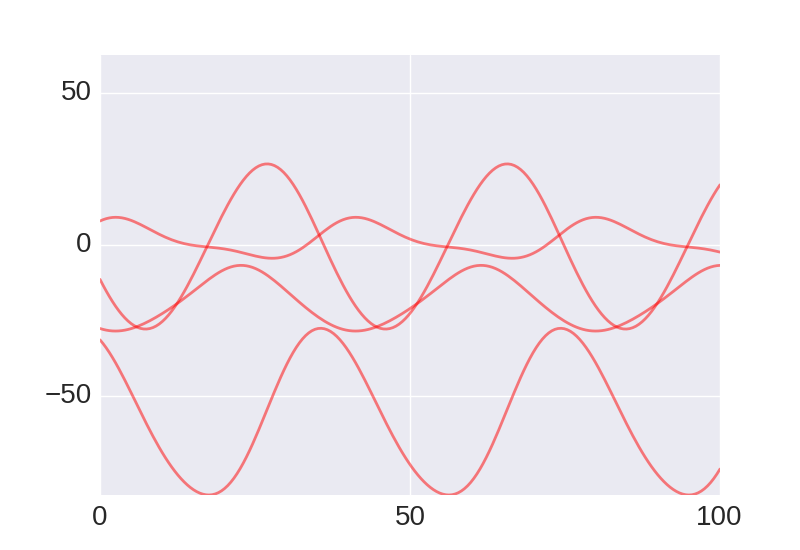
\includegraphics[width=\textwidth]{figs/composition/composition_demo_PER_prior.png}
        \caption{PER}
    \end{subfigure}
    ~ %add desired spacing between images, e. g. ~, \quad, \qquad, \hfill etc. 
    %(or a blank line to force the subfigure onto a new line)
    \begin{subfigure}[b]{0.3\textwidth}
        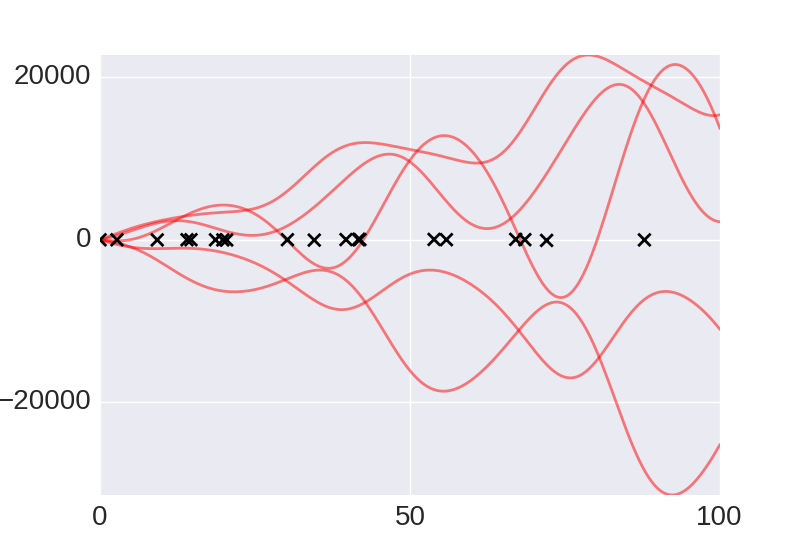
\includegraphics[width=\textwidth]{figs/composition/composition_demo_LINxPER_prior.png}
        \caption{LIN $\times$ PER}
    \end{subfigure} \vspace{4mm} 

Posterior:

 \begin{subfigure}[b]{0.3\textwidth}
        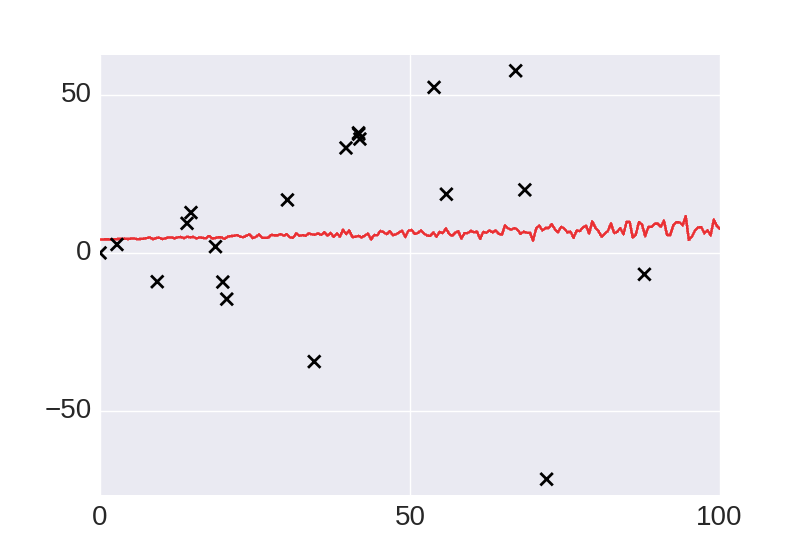
\includegraphics[width=\textwidth]{figs/composition/composition_demo_LIN.png}
        \caption{LIN}
    \end{subfigure}
    ~ %add desired spacing between images, e. g. ~, \quad, \qquad, \hfill etc. 
      %(or a blank line to force the subfigure onto a new line)
    \begin{subfigure}[b]{0.3\textwidth}
        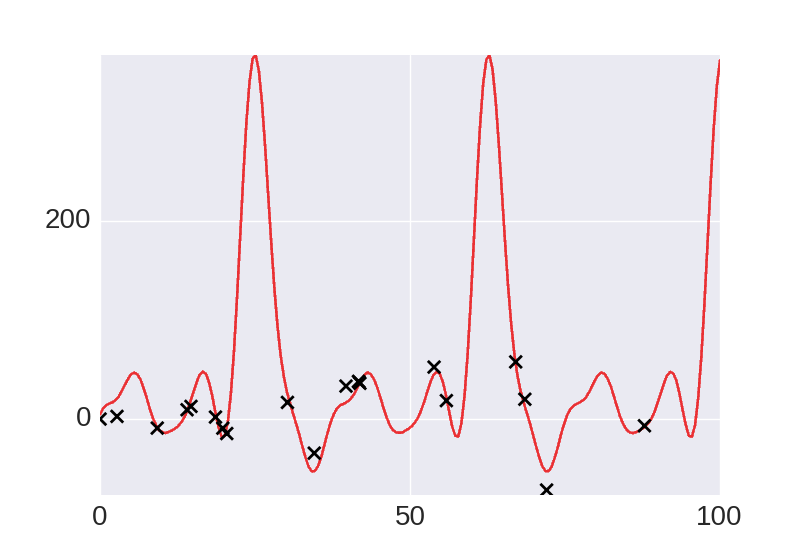
\includegraphics[width=\textwidth]{figs/composition/composition_demo_PER.png}
        \caption{PER}
    \end{subfigure}
    ~ %add desired spacing between images, e. g. ~, \quad, \qquad, \hfill etc. 
    %(or a blank line to force the subfigure onto a new line)
    \begin{subfigure}[b]{0.3\textwidth}
        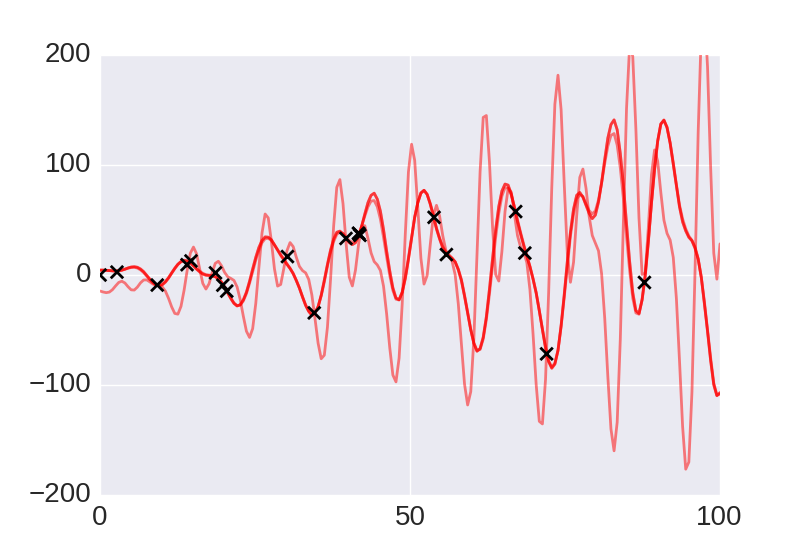
\includegraphics[width=\textwidth]{figs/composition/composition_demo_LINxPER.png}
        \caption{LIN $\times$ PER}
    \end{subfigure}

%20.0739791735
%6.31647597198
%37.7184218042
%19.1051376016

\caption{Kernel composition}
\end{figure}


The covariance function (or kernel) of a \ac{GP} governs high-level properties of the observed data such as linearity, periodicity and smoothness.
It comes with few free parameters that we call hyper-parameters.
Adjusting the hyper-parameters changes non-qualitative attributes such as length
scales while preserving the qualitative properties of the distribution.
More drastically different covariance functions are achieved by changing the structure of the covariance function itself.
%A different type could be a linear covariance function:
%\begin{equation}
% k(x,x^\prime) = \sigma^2 (x-\ell) (x^\prime-\ell). 
%\end{equation}
Note that covariance function structures are compositional: adding or multiplying two valid covariance functions results in another valid covariance function. 







Venture includes the primitive \texttt{make\_gp}, which takes as arguments a
unary function \texttt{mean} and a binary (symmetric, positive-semidefinite)
function \texttt{cov} and produces a function $\gtt$ distributed as a Gaussian
process with the supplied mean and covariance.  For example, a function $\gtt
\sim \GP(0,\,\SE)$, where $\SE$ is a squared-exponential covariance
\[ \SE(x, x') = \sigma^2 \exp\pn{\frac{(x-x')^2}{2\ell}} \]
with $\sigma=1$ and $\ell=1$, can be instantiated as follows:
\begin{lstlisting}[language=Venture]
assume zero = make_const_func( 0.0)
assume se = make_squaredexp( 1.0, 1.0)
assume g  = make_gp( zero, se)
\end{lstlisting}
There are two ways two view $\gtt$ as a ``random function.'' In the first view,
the \texttt{assume} directive that instantiates $\gtt$ does not use any
randomness---only the subsequent calls to $\gtt$ do---and coherence constraints
are upheld by the interpreter by keeping track of which evaluations of $\gtt$
exist in the current execution trace.  Namely, if the current trace contains evaluations
of $\gtt$ at the points $x_1,\ldots,x_N$ with return values $y_1,\ldots,y_N$,
then the next evaluation of $\gtt$ (say, jointly at the points $x_{N+1}, \ldots,
x_{N+n}$) will be distributed according to the joint conditional distribution
\[
  P\pn{\big.
    \texttt(\gtt\ x_{N+1}\texttt), \ldots, \texttt(\gtt\ x_{N+n}\texttt)
    \mvert
    \texttt(\gtt\ x_i\texttt) = f_i \text{ for $i=1,\ldots,N$}}.
\]
In the second view, $\gtt$ is a randomly chosen deterministic function, chosen
from the space of all deterministic real-valued functions; in this view, the
\texttt{assume} directive contains \emph{all} the randomness, and subsequent
invocations of $\gtt$ are deterministic.  The first view is procedural and is
faithful to the computation that occurs behind the scenes in Venture.  The
second view is declarative and is faithful to notations like ``$g \sim P(g)$''
which are often used in mathematical treatments.  Because a model program could
make arbitrarily many calls to $\gtt$, and the joint distribution on the return
values of the calls could have arbitrarily high entropy, it is not
computationally possible in finite time to choose the entire function $\gtt$ all
at once as in the second view.  Thus, it stands to reason that any
computationally implementable notion of ``nonparametric random functions'' must
involve incremental random choices in one way or another, and \ac{GP}s
in Venture are no exception.
